\documentclass[a4paper,oneside,12pt]{report}
% Package yang diperlukan
\usepackage{fontspec}       % Font sistem untuk XeLaTeX/LuaLaTeX
\usepackage{setspace}       % Pengaturan jarak antarbaris
\usepackage{graphicx}      % Untuk memasukkan gambar
\usepackage{titling}       % Untuk kustomisasi halaman judul
\usepackage{geometry}      % Untuk mengatur margin halaman
\usepackage{listings}      % Untuk menampilkan blok kode
\usepackage{xcolor}        % Untuk menggunakan warna
\usepackage{float}         % Untuk kontrol penempatan float (seperti gambar)
\usepackage{xurl}          % Untuk pemutusan tautan URL yang lebih baik
\usepackage{hyperref}      % Untuk membuat hyperlink (URL, referensi)
\usepackage{indentfirst}   % Untuk memberi indentasi pada paragraf pertama setiap seksi
\usepackage{url}           % Untuk format URL
\usepackage{fancyhdr}      % Untuk kustomisasi header dan footer
\usepackage{tocloft}       % Untuk kustomisasi Daftar Isi
\usepackage{bookmark}      % Untuk manajemen bookmark PDF yang lebih baik
\usepackage{amsmath}       % Untuk rumus matematika
\usepackage{amssymb}       % Untuk simbol matematika
\usepackage{booktabs}      % Untuk tabel yang lebih rapi
\usepackage{caption}
\usepackage{subcaption}    % Untuk tata letak gambar berdampingan
\usepackage{tabularx}      % Untuk tabel dengan lebar otomatis sesuai margin
\usepackage{array}         % Untuk kontrol kolom tabel
\usepackage{enumitem}      % Untuk kontrol kerapatan daftar
\usepackage[none]{hyphenat} % Nonaktifkan seluruh pemotongan kata bertanda hubung
\usepackage{microtype}     % Tipografi halus dan protrusion antislop

% Font dan spasi standar laporan praktikum
\setmainfont{Times New Roman}
\onehalfspacing

%======================================================================
% PENGATURAN GEOMETRI HALAMAN
%======================================================================
\geometry{left=3cm, right=2.5cm, top=2cm, bottom=2.5cm}
\sloppy
\tolerance=10000
\emergencystretch=3em
\hfuzz=1.5pt
\hbadness=10000
\hyphenpenalty=10000
\exhyphenpenalty=10000
\righthyphenmin=62
\lefthyphenmin=62

%======================================================================
% PENGATURAN WARNA UNTUK BLOK KODE
%======================================================================
\definecolor{codegreen}{rgb}{0,0.6,0}
\definecolor{codegray}{rgb}{0.5,0.5,0.5}
\definecolor{codepurple}{rgb}{0.58,0,0.82}
\definecolor{backcolour}{rgb}{0.95,0.95,0.92}
\definecolor{darkblue}{rgb}{0,0,0.6}

%======================================================================
% PENGATURAN BLOK KODE (LISTINGS)
%======================================================================
\lstdefinestyle{commonstyle}{
    backgroundcolor=\color{backcolour},
    breakatwhitespace=false,
    breaklines=true,
    captionpos=b,
    keepspaces=true,
    numbers=left,
    numbersep=5pt,
    showspaces=false,
    showstringspaces=false,
    showtabs=false,
    tabsize=2,
    frame=single,
    basicstyle=\ttfamily\scriptsize,
    numberstyle=\tiny\color{codegray},
    columns=flexible,
    postbreak=\mbox{\textcolor{red}{$\hookrightarrow$}\space},
    breakindent=0pt,
    breakautoindent=false
}
\lstdefinestyle{pythonstyle}{
    style=commonstyle,
    language=Python,
    commentstyle=\color{codegreen},
    keywordstyle=\color{darkblue},
    stringstyle=\color{codepurple},
    emph={import,from,class,def,for,while,if,else,elif,try,except,finally},
    emphstyle=\color{darkblue}
}

%======================================================================
% PENGATURAN LAIN-LAIN
%======================================================================
\newcommand{\customfbox}[1]{%
  \setlength{\fboxsep}{0pt}%
  \setlength{\fboxrule}{0.5pt}%
  \fcolorbox{black}{white}{#1}%
}
\renewcommand{\figurename}{Gambar}
\renewcommand{\thefigure}{\arabic{figure}}
\renewcommand{\tablename}{Tabel}
\renewcommand{\thetable}{\arabic{table}}
\renewcommand{\theequation}{\arabic{equation}}
\renewcommand{\lstlistingname}{Listing}
\AtBeginDocument{\renewcommand{\thelstlisting}{\arabic{lstlisting}}}
\counterwithout{figure}{chapter}
\counterwithout{table}{chapter}
\counterwithout{equation}{chapter}
\hypersetup{
    colorlinks=true,
    linkcolor=black,
    filecolor=black,
    urlcolor=black,
    citecolor=black,
    pdftitle={Laporan Praktikum Penambangan Data Pertemuan 9},
    pdfpagemode=FullScreen,
    breaklinks=true
}
\pagestyle{fancy}
\fancyhf{}
\fancyfoot[C]{\thepage}
\renewcommand{\headrulewidth}{0pt}
\fancypagestyle{plain}{
    \fancyhf{}
    \fancyfoot[C]{\thepage}
    \renewcommand{\headrulewidth}{0pt}
}
\renewcommand{\contentsname}{Daftar Isi}
\renewcommand{\bibname}{Daftar Pustaka}
\renewcommand{\thechapter}{}
\renewcommand{\chaptername}{}
\renewcommand{\thesection}{\arabic{chapter}.\arabic{section}}
\renewcommand{\thesubsection}{\thesection.\arabic{subsection}}
\setcounter{secnumdepth}{3}
\setcounter{tocdepth}{3}
\renewcommand{\cftchapdotsep}{\cftdotsep}
\renewcommand{\cftchapleader}{\cftdotfill{\cftchapdotsep}}
\setlength{\cftchapindent}{0em}
\setlength{\cftsecindent}{2em}
\setlength{\cftsubsecindent}{4em}
\setlength{\cftchapnumwidth}{0em}
\setlength{\cftsecnumwidth}{2.5em}
\setlength{\cftsubsecnumwidth}{3.2em}
\setlength{\cftbeforechapskip}{4pt}
\setlength{\cftbeforesecskip}{1.5pt}
\setlength{\cftbeforesubsecskip}{0.5pt}
\renewcommand{\cftchappresnum}{}
\renewcommand{\cftchapaftersnum}{}
\newcommand{\tocboldsection}[1]{%
  \protect\renewcommand{\protect\cftchapfont}{\protect\bfseries}%
  #1%
  \protect\renewcommand{\protect\cftchapfont}{}%
}

%======================================================================
% AWAL DOKUMEN
%======================================================================
\begin{document}

% Halaman Judul
\newgeometry{left=3cm, right=2.5cm, top=2.5cm, bottom=3cm}
\begin{titlingpage}
	\begin{spacing}{1}
		\begin{center}
			\vspace*{0.2cm}
			{\large \textbf{\MakeUppercase{Laporan Praktikum}}} \\[0.4cm]
			{\large \textbf{\MakeUppercase{Praktikum Penambangan Data}}} \\[0.4cm]
			{\large \textbf{\MakeUppercase{Pertemuan 9}}} \\[0.4cm]
			{\large \textbf{\MakeUppercase{Convolutional Neural Network}}} \\[1.5cm]

			
\includegraphics[height=7cm]{images/UGM.png} \\[0.7cm]

			{\normalsize \textbf{Disusun oleh:}} \\[0.4cm]
			\begin{tabular}{@{}l l @{}}
				\textbf{Nama}           & : Hafidz Rizqullah Prasetya        \\
				\textbf{NIM}            & : 24/535493/SV/24243               \\
				\textbf{Kelas}          & : PL5A1                            \\
				\textbf{Dosen Pengampu} & : Dr. Imam Fahrurrozi, S.T., M.Cs.
			\end{tabular} \\[1.2cm]

			{\normalsize \textbf{PROGRAM STUDI D-IV}} \\[0.2cm]
			{\normalsize \textbf{TEKNOLOGI REKAYASA PERANGKAT LUNAK}} \\[0.2cm]
			{\normalsize \textbf{DEPARTEMEN TEKNIK ELEKTRO DAN INFORMATIKA}} \\[0.2cm]
			{\normalsize \textbf{SEKOLAH VOKASI}} \\[0.2cm]
			{\normalsize \textbf{UNIVERSITAS GADJAH MADA}} \\[0.2cm]
			{\normalsize \textbf{YOGYAKARTA}} \\[0.2cm]
			{\normalsize \textbf{2026}} \\[1.2cm]
		\end{center}
	\end{spacing}
\end{titlingpage}
\restoregeometry

\thispagestyle{empty}
\clearpage
\stepcounter{page}
\thispagestyle{empty}

% --- Daftar Isi ---
\addcontentsline{toc}{chapter}{Daftar Isi}
\begin{spacing}{0.92}
	\tableofcontents
\end{spacing}
\clearpage

% Mengatur penomoran halaman menjadi arab dan mulai dari 3
\pagenumbering{arabic}
\setcounter{page}{3}

\chapter[Tujuan Praktikum]{Tujuan Praktikum}
Berdasarkan Modul Pertemuan 9 Praktikum Penambangan Data, tujuan praktikum ini adalah:
\begin{enumerate}[noitemsep, topsep=4pt, parsep=2pt]
	\item Memahami keterbatasan \textit{Multi-Layer Perceptron} (MLP) saat mengolah citra digital dan keunggulan arsitektur \textit{Convolutional Neural Network} (CNN).
	\item Menjelaskan komponen dasar CNN, yaitu \textit{convolution layer}, fungsi aktivasi ReLU, \textit{pooling layer}, \textit{flattening}, dan \textit{fully connected layer} (\textit{dense}).
	\item Membangun model CNN sederhana menggunakan \textit{framework} Keras dan TensorFlow.
	\item Menerapkan regularisasi \textit{dropout} untuk mencegah \textit{overfitting}.
\end{enumerate}

\clearpage

\chapter{Dasar Teori}

\section{Representasi Citra Digital dan Keterbatasan MLP}
Komputer membaca citra sebagai matriks piksel. Citra berwarna berukuran $224 \times 224$ disimpan sebagai \textit{array} berdimensi $224 \times 224 \times 3$, dengan tiga kanal warna merah, hijau, dan biru (RGB). Setiap elemen bernilai bulat 0 sampai 255 yang menyatakan intensitas cahaya pada kanal tersebut \cite{goodfellow2016}. Klasifikasi citra sendiri termasuk tugas klasifikasi dalam penambangan data, yaitu memetakan objek ke salah satu label kelas berdasarkan fitur yang dimilikinya \cite{han2022}.

Kalau citra seperti ini langsung dimasukkan ke MLP, ada dua masalah yang muncul. Masalah pertama adalah jumlah parameter yang membengkak (\textit{parameter explosion}). Satu citra $224 \times 224 \times 3$ menghasilkan 150.528 nilai masukan, sehingga satu \textit{hidden layer} berisi 1.000 neuron saja sudah membutuhkan sekitar 150 juta bobot. Masalah kedua adalah hilangnya informasi spasial. MLP mewajibkan citra diratakan menjadi vektor satu dimensi, sehingga hubungan ketetanggaan antarpiksel hilang. Akibatnya MLP mudah gagal ketika objek bergeser, berubah skala, atau berotasi sedikit \cite{lecun1998}.

\section{Convolutional Neural Network (CNN)}
CNN adalah jenis \textit{feed-forward neural network} yang dirancang untuk data berbentuk \textit{grid}, terutama citra. CNN belajar mengekstrak pola visual secara bertingkat langsung dari piksel mentah, mulai dari tepi dan tekstur pada lapisan awal sampai bentuk objek pada lapisan yang lebih dalam \cite{oshea2015}. Ada dua gagasan yang membuat CNN hemat parameter: \textit{local connectivity} (setiap neuron hanya melihat sebagian kecil citra) dan \textit{weight sharing} (filter yang sama dipakai di seluruh posisi citra) \cite{lecun1998}.

\subsection{Convolution Layer}
Lapisan konvolusi memakai sejumlah filter atau \textit{kernel} berukuran kecil, misalnya $3 \times 3$, yang digeser (\textit{stride}) di atas citra masukan. Pada setiap posisi, filter menghitung perkalian titik (\textit{dot product}) dengan potongan citra di bawahnya. Untuk citra masukan $I$ dan kernel $K$ berukuran $k \times k$, nilai \textit{feature map} pada posisi $(i, j)$ adalah:
\begin{equation}
	S(i, j) = \sum_{m=0}^{k-1} \sum_{n=0}^{k-1} I(i+m, j+n)\, K(m, n) + b
\end{equation}
Setiap filter menghasilkan satu \textit{feature map}. Jumlah parameter satu lapisan \texttt{Conv2D} dihitung dengan $(k \cdot k \cdot C_{in} + 1) \cdot C_{out}$, dengan $C_{in}$ jumlah kanal masukan dan $C_{out}$ jumlah filter. Opsi \texttt{padding='same'} menambahkan nilai nol di tepi citra agar ukuran keluaran sama dengan masukan \cite{keras-conv2d}.

\subsection{Fungsi Aktivasi ReLU}
Setelah konvolusi, nilai \textit{feature map} dilewatkan ke fungsi aktivasi \textit{Rectified Linear Unit} (ReLU):
\begin{equation}
	\Phi(x) = \max(0, x)
\end{equation}
ReLU mengubah semua nilai negatif menjadi nol dan meneruskan nilai positif apa adanya. Fungsi ini membuat jaringan mampu memodelkan hubungan non-linier dan komputasinya murah \cite{krizhevsky2012}.

\subsection{Pooling Layer}
\textit{Pooling} mengecilkan ukuran spasial (lebar dan tinggi) \textit{feature map} sehingga beban komputasi berkurang dan model lebih tahan terhadap pergeseran kecil (\textit{translation invariance}). Jenis yang paling sering dipakai adalah \textit{max pooling}, yaitu mengambil nilai terbesar dalam jendela tertentu. \textit{Max pooling} $2 \times 2$ memperkecil \textit{feature map} $112 \times 112$ menjadi $56 \times 56$ tanpa menambah parameter \cite{goodfellow2016}.

\subsection{Flattening dan Fully Connected Layer}
\textit{Flattening} mengubah \textit{feature map} tiga dimensi dari lapisan \textit{pooling} terakhir menjadi satu vektor. Vektor ini diteruskan ke \textit{fully connected layer} (\textit{dense}) yang berperan sebagai pengklasifikasi. Lapisan keluaran memakai aktivasi \textit{softmax} agar menghasilkan probabilitas untuk setiap kelas:
\begin{equation}
	\sigma(z)_i = \frac{e^{z_i}}{\sum_{j=1}^{K} e^{z_j}}
\end{equation}
dengan $K$ jumlah kelas \cite{oshea2015}.

\section{Regularisasi Dropout}
\textit{Dropout} adalah teknik regularisasi yang menonaktifkan sebagian neuron secara acak dengan probabilitas $p$ pada setiap langkah pelatihan. Neuron yang dimatikan tidak ikut dalam \textit{forward pass} maupun \textit{backward pass} pada langkah tersebut. Cara ini mencegah neuron saling bergantung secara berlebihan (\textit{co-adaptation}), sehingga jaringan dipaksa mempelajari fitur yang lebih umum. Saat inferensi, semua neuron aktif kembali \cite{srivastava2014}. Di Keras, lapisan \texttt{Dropout} hanya aktif ketika model sedang dilatih \cite{keras-dropout}.

\section{Fungsi Loss, Optimizer, dan Metrik Evaluasi}
Untuk klasifikasi multi-kelas, fungsi kerugian yang dipakai adalah \textit{categorical cross-entropy}:
\begin{equation}
	\mathcal{L} = -\sum_{i=1}^{K} y_i \log(\hat{y}_i)
\end{equation}
dengan $y_i$ label aktual dalam bentuk \textit{one-hot} dan $\hat{y}_i$ probabilitas prediksi. Varian \texttt{sparse\_categorical\_crossentropy} menghitung hal yang sama tetapi menerima label berupa bilangan bulat. Bobot diperbarui oleh \textit{optimizer} seperti RMSprop atau Adam \cite{goodfellow2016}.

Performa klasifikasi saya ukur dengan \textit{accuracy}, \textit{precision}, \textit{recall}, dan \textit{F1-score} untuk setiap kelas, ditambah \textit{confusion matrix} yang membandingkan label aktual dengan label prediksi:
\begin{align}
	\text{Precision} & = \frac{TP}{TP + FP}, \qquad \text{Recall} = \frac{TP}{TP + FN} \\
	\text{F1-Score}  & = \frac{2 \cdot \text{Precision} \cdot \text{Recall}}{\text{Precision} + \text{Recall}}
\end{align}

\clearpage

\chapter{Alat dan Bahan}

\section{Perangkat Keras}
\begin{enumerate}[noitemsep, topsep=2pt, parsep=1pt]
	\item Laptop dengan prosesor 12 \textit{thread} dan RAM 14 GB.
	\item Koneksi internet untuk mengunduh dataset.
\end{enumerate}

\section{Perangkat Lunak}
\begin{enumerate}[noitemsep, topsep=2pt, parsep=1pt]
	\item Sistem operasi Linux 64-bit.
	\item Jupyter Notebook lokal (notebook juga dapat dijalankan di Google Colaboratory).
	\item Python 3.12.
	\item Pustaka Python:
	      \begin{itemize}[noitemsep, topsep=1pt, parsep=0.5pt]
		      \item \texttt{tensorflow} 2.21 (versi CPU) dan \texttt{keras} 3.15: membangun dan melatih CNN.
		      \item \texttt{numpy}: manipulasi \textit{array} citra.
		      \item \texttt{matplotlib} dan \texttt{seaborn}: menampilkan citra, grafik, dan \textit{heatmap}.
		      \item \texttt{scikit-learn}: \texttt{classification\_report} dan \texttt{confusion\_matrix}.
	      \end{itemize}
\end{enumerate}

\section{Dataset}
\begin{enumerate}[noitemsep, topsep=2pt, parsep=1pt]
	\item Dataset \textit{Dog vs Cat} dari modul, berisi 100 citra JPEG (50 kucing dan 50 anjing).
	\item Dataset CIFAR-10 \cite{krizhevsky2009}, berisi 60.000 citra berwarna $32 \times 32$ piksel dalam 10 kelas, dimuat lewat \texttt{tf.keras.datasets.cifar10}.
\end{enumerate}

\clearpage

\chapter[\texorpdfstring{\tocboldsection{Hasil dan Pembahasan}}{Hasil dan Pembahasan}]{Hasil dan Pembahasan}

Seluruh percobaan saya jalankan di Jupyter Notebook lokal memakai CPU. Notebook lengkap beserta keluarannya dapat dibuka di Google Colaboratory melalui tautan berikut:

\begin{center}
	\href{https://colab.research.google.com/github/hafidzrizqullahprasetya/PPD/blob/main/pertemuan-9/praktikum-9-convolutional-neural-network.ipynb}{\textcolor{blue}{\url{https://colab.research.google.com/github/hafidzrizqullahprasetya/PPD/blob/main/pertemuan-9/praktikum-9-convolutional-neural-network.ipynb}}} \cite{colab-notebook}
\end{center}

\section{Percobaan Modul: Klasifikasi Citra Dog vs Cat}

\subsection{Unduh Dataset}
Modul memakai perintah \texttt{gdown} di Colab. Supaya notebook bisa jalan di Colab maupun lokal tanpa paket tambahan, saya mengunduh berkas ZIP dengan \texttt{urllib}, mengekstraknya, lalu memindahkan citra ke folder \texttt{dataset/cat} dan \texttt{dataset/dog}.

\begin{figure}[H]
	\centering
	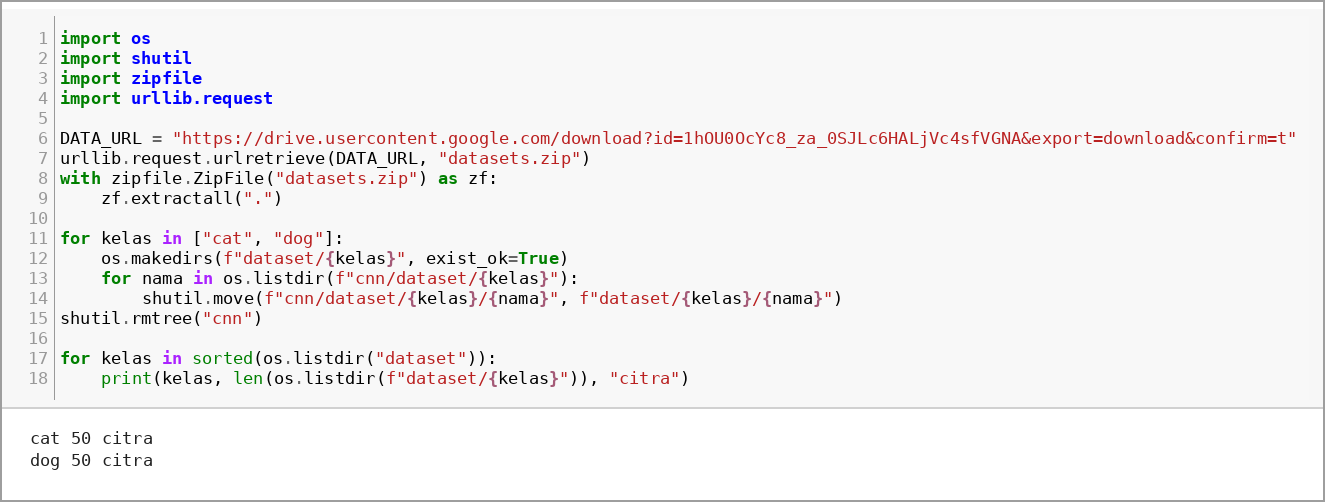
\includegraphics[width=0.85\textwidth]{images/ss-01-unduh-dataset.png}
	\caption{Kode unduh dan ekstraksi dataset Dog vs Cat beserta jumlah citra per kelas.}
	\label{fig:ss-unduh}
\end{figure}

Keluaran sel menunjukkan masing-masing kelas berisi 50 citra, jadi dataset ini seimbang.

\subsection{Impor Pustaka}
Pustaka yang saya impor sama dengan modul, yaitu \texttt{tensorflow}, \texttt{matplotlib}, \texttt{numpy}, serta lapisan \texttt{Conv2D}, \texttt{MaxPooling2D}, \texttt{Dropout}, \texttt{Flatten}, dan \texttt{Dense}. Saya menambahkan \textit{seed} 42 untuk \texttt{random}, \texttt{numpy}, dan TensorFlow agar hasil pembagian data dan inisialisasi bobot lebih mudah diulang.

\begin{figure}[H]
	\centering
	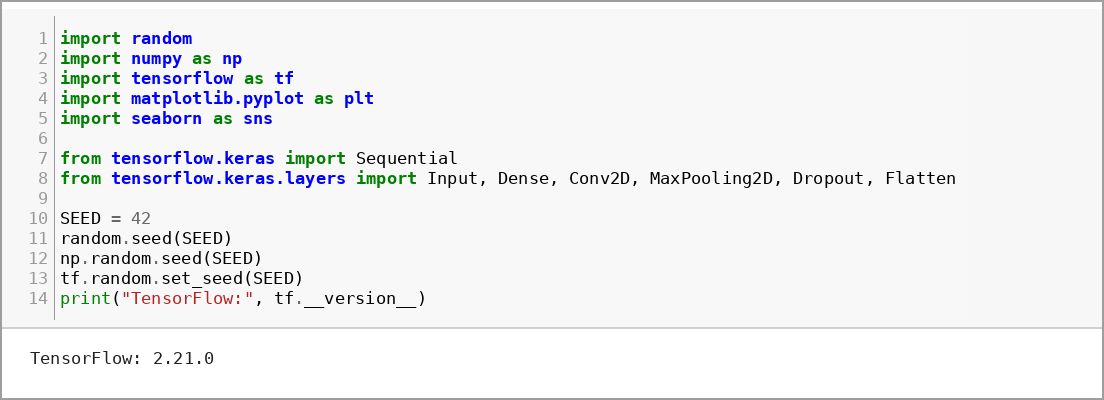
\includegraphics[width=0.8\textwidth]{images/ss-02-impor-pustaka.png}
	\caption{Impor pustaka dan pengaturan \textit{seed}.}
	\label{fig:ss-impor}
\end{figure}

\subsection{Pembacaan dan Pembagian Dataset}
Citra dibaca dengan \texttt{ImageDataGenerator} lalu \texttt{flow\_from\_directory}. Semua citra diubah ukurannya menjadi $224 \times 224$ piksel dan nilai pikselnya dibagi 255 (\texttt{rescale=1./255}) agar berada di rentang 0 sampai 1. Parameter \texttt{validation\_split=0.2} membagi data menjadi 80\% latih dan 20\% validasi.

\begin{lstlisting}[style=pythonstyle,caption={Pembacaan dan pembagian dataset Dog vs Cat.}]
IMAGE_SIZE = 224
BATCH_SIZE = 16

datagen = tf.keras.preprocessing.image.ImageDataGenerator(
    rescale=1. / 255,
    validation_split=0.2)

train_generator = datagen.flow_from_directory(
    base_dir, target_size=(IMAGE_SIZE, IMAGE_SIZE),
    batch_size=BATCH_SIZE, subset='training', seed=SEED)
\end{lstlisting}

\begin{figure}[H]
	\centering
	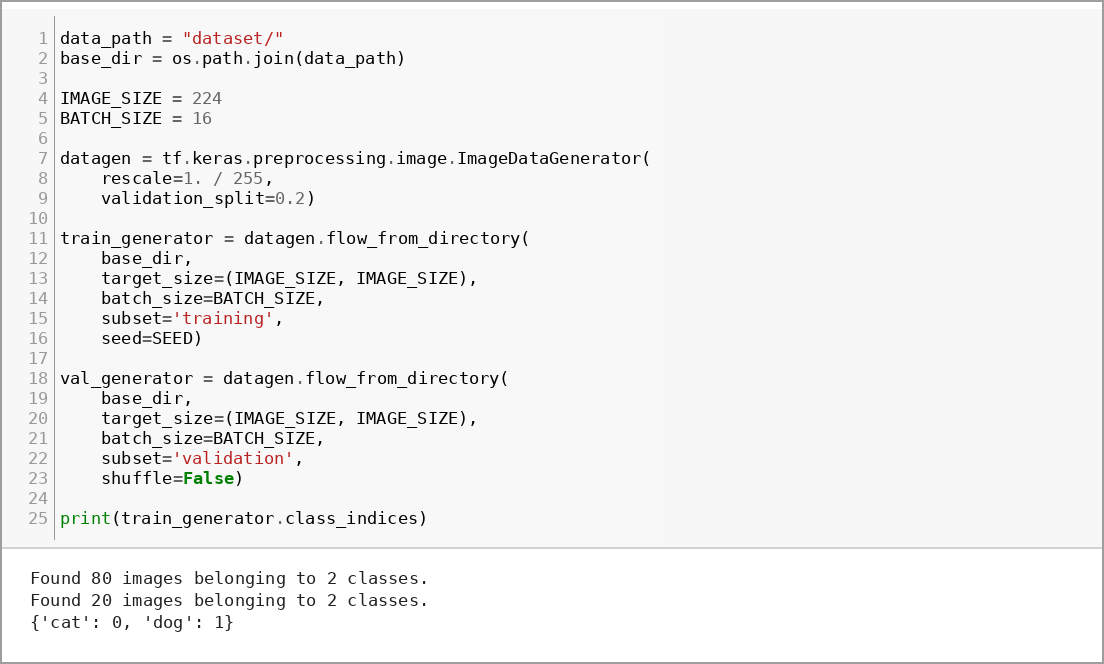
\includegraphics[width=0.8\textwidth]{images/ss-03-split-dataset.png}
	\caption{Pembagian dataset menjadi 80 citra latih dan 20 citra validasi.}
	\label{fig:ss-split}
\end{figure}

Hasilnya 80 citra latih dan 20 citra validasi, sama dengan keluaran pada modul. Kelas \texttt{cat} diberi indeks 0 dan \texttt{dog} indeks 1. Ukuran \textit{batch} saya turunkan dari 64 (modul) menjadi 16 karena pelatihan berjalan di CPU dengan RAM terbatas. Satu \textit{batch} 64 citra $224 \times 224$ dengan 32 filter menghasilkan aktivasi sekitar 400 MB per lapisan konvolusi, dan model ini punya empat lapisan konvolusi.

\subsection{Uji Coba Pembacaan Data}
Saya mengambil satu \textit{batch} dari \texttt{train\_generator} lalu menampilkan delapan citra pertama beserta labelnya.

\begin{figure}[H]
	\centering
	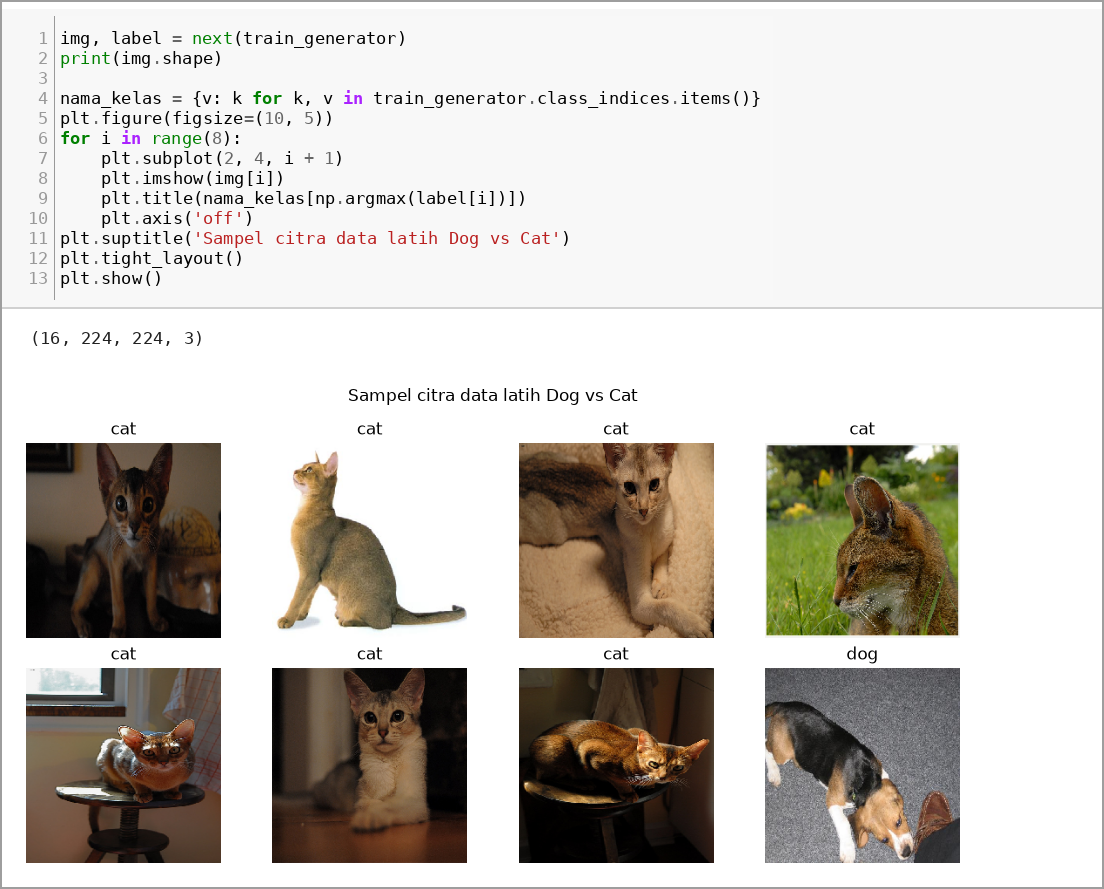
\includegraphics[width=0.8\textwidth]{images/ss-04-sampel-citra.png}
	\caption{Sampel citra data latih Dog vs Cat beserta labelnya.}
	\label{fig:ss-sampel}
\end{figure}

Bentuk \textit{batch} yang terbaca adalah \texttt{(16, 224, 224, 3)}, artinya 16 citra berwarna $224 \times 224$. Label pada judul setiap citra sesuai dengan isi gambarnya, jadi pipeline data sudah benar. Terlihat juga bahwa latar, pencahayaan, dan pose hewan sangat beragam, sehingga tugas ini cukup sulit untuk model yang hanya dilatih dengan 80 citra.

\subsection{Cek Bentuk Data dan IMG\_SHAPE}
\begin{figure}[H]
	\centering
	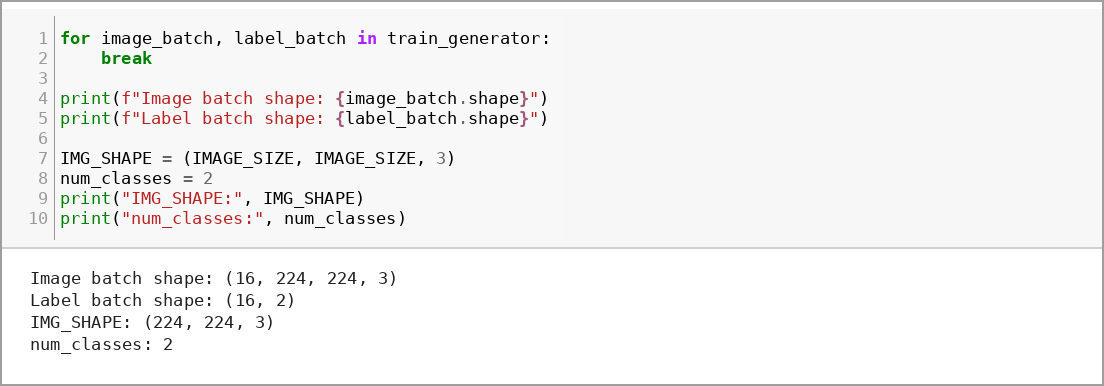
\includegraphics[width=0.8\textwidth]{images/ss-05-img-shape.png}
	\caption{Pemeriksaan bentuk \textit{batch} dan pendefinisian \texttt{IMG\_SHAPE}.}
	\label{fig:ss-imgshape}
\end{figure}

Bentuk label \texttt{(16, 2)} menunjukkan label sudah dalam format \textit{one-hot} dua kelas (bawaan \texttt{class\_mode='categorical'}). Karena itu lapisan keluaran memakai dua neuron \textit{softmax} dan fungsi loss \texttt{categorical\_crossentropy}. Variabel \texttt{IMG\_SHAPE} saya tetapkan \texttt{(224, 224, 3)} dan \texttt{num\_classes = 2}.

\subsection{Membangun Model CNN Sederhana}
Arsitektur mengikuti modul: dua blok konvolusi, masing-masing berisi dua \texttt{Conv2D} dan satu \texttt{MaxPooling2D}. Blok pertama memakai 32 filter dan diikuti \texttt{Dropout(0.1)}, blok kedua memakai 64 filter. Bagian pengklasifikasi saya ubah dari \texttt{Dense(512)} menjadi \texttt{Dense(128)} yang diikuti \texttt{Dropout(0.5)}. Alasannya, keluaran \texttt{Flatten} berukuran 200.704, sehingga \texttt{Dense(512)} akan membutuhkan sekitar 102 juta bobot dan tidak muat di memori laptop saya saat pelatihan.

\begin{figure}[H]
	\centering
	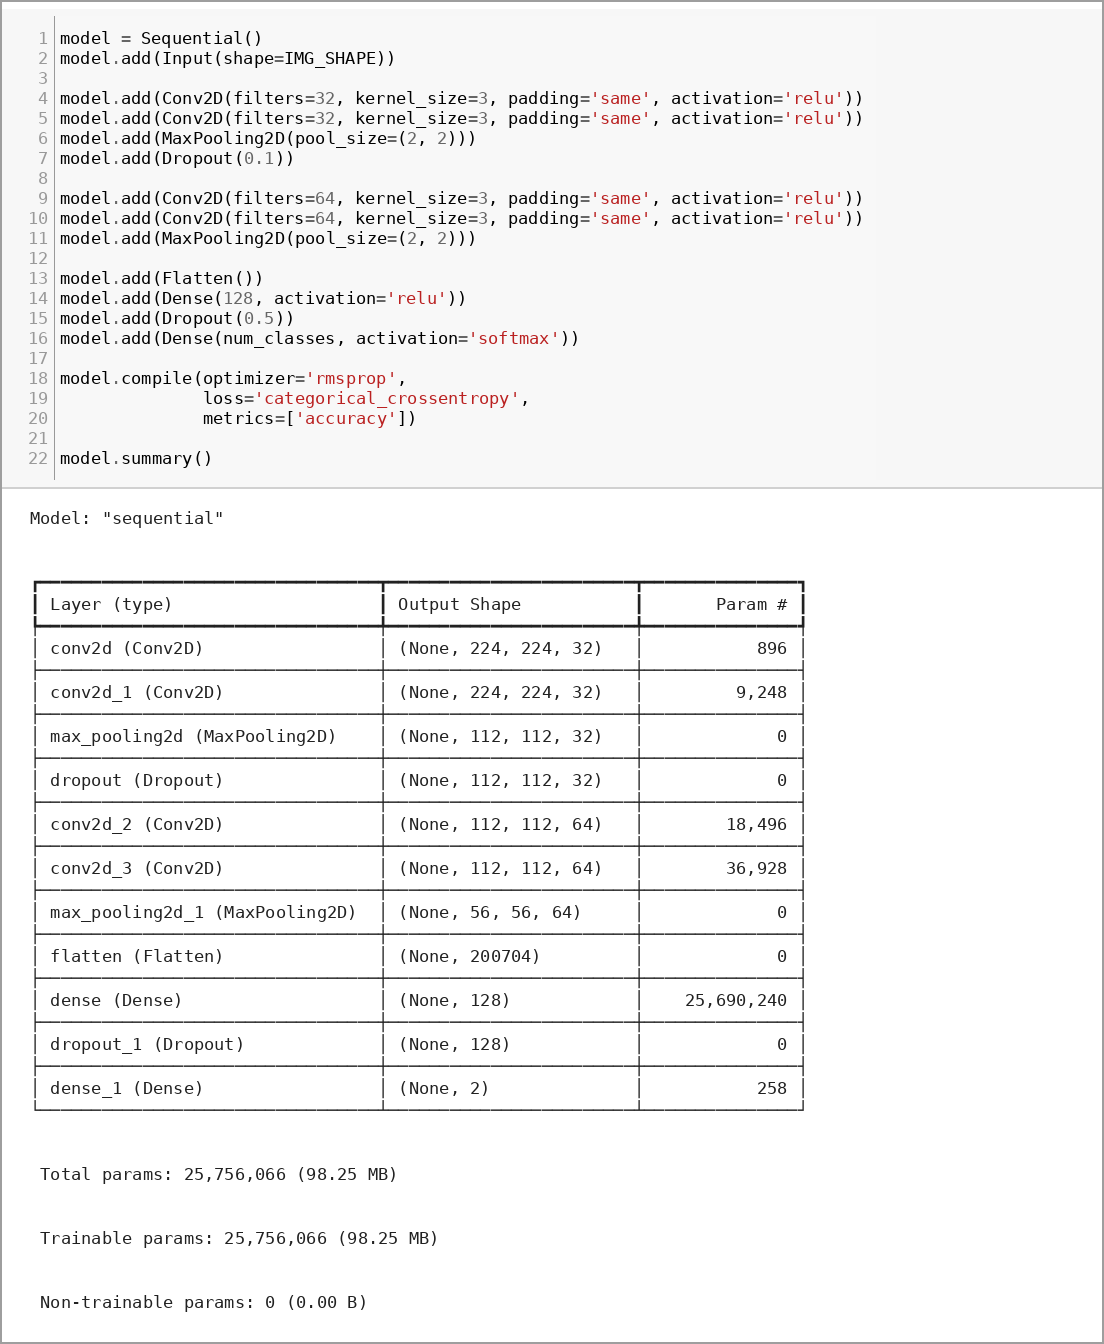
\includegraphics[width=0.78\textwidth]{images/ss-06-model-cnn-summary.png}
	\caption{Kode arsitektur CNN sederhana dan ringkasan \texttt{model.summary()}.}
	\label{fig:ss-summary}
\end{figure}

Dari ringkasan model, total parameternya 25.756.066 (98,25 MB). Yang menarik, keempat lapisan konvolusi hanya menyumbang 65.568 parameter, sedangkan lapisan \texttt{dense} pertama sendirian menyumbang 25.690.240 parameter atau sekitar 99,7\% dari total. Ini membuktikan poin pada dasar teori: konvolusi dengan \textit{weight sharing} sangat hemat parameter, dan beban terbesar justru muncul di lapisan \textit{fully connected} setelah \textit{flatten}.

\subsection{Melatih Model}
Model dilatih selama 20 \textit{epoch} dengan \textit{optimizer} RMSprop sesuai modul.

\begin{figure}[H]
	\centering
	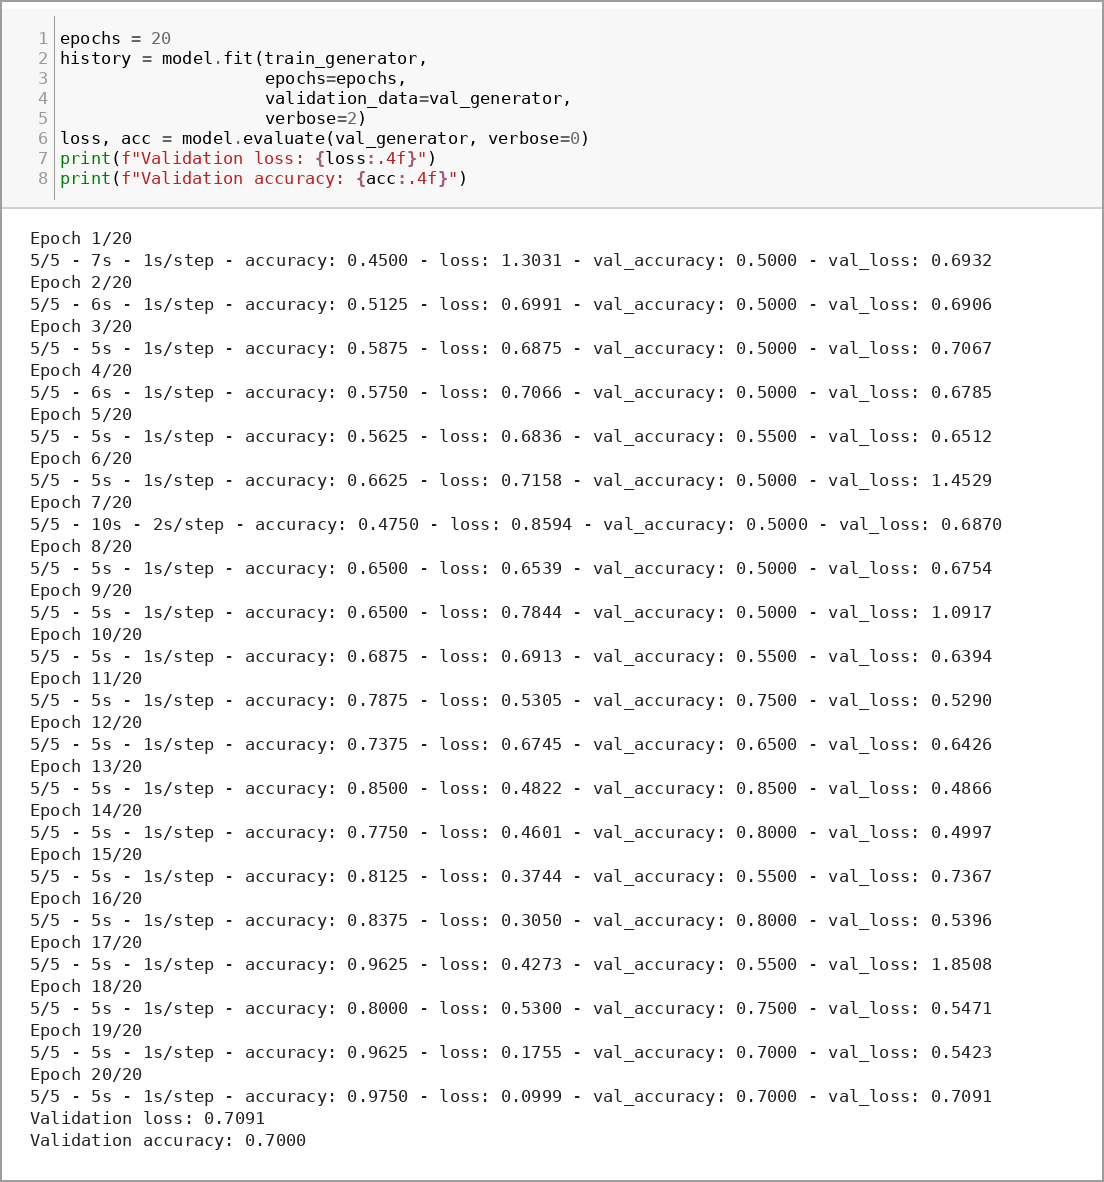
\includegraphics[width=0.8\textwidth]{images/ss-07-latih-model.png}
	\caption{Log pelatihan model CNN Dog vs Cat selama 20 \textit{epoch}.}
	\label{fig:ss-latih}
\end{figure}

Selama 10 \textit{epoch} pertama, akurasi validasi tertahan di 0,50 (setara tebakan acak) walaupun akurasi latih naik turun di kisaran 0,45 sampai 0,69. Model baru mulai belajar pola yang berguna pada \textit{epoch} 11, ketika akurasi validasi naik ke 0,75, lalu mencapai nilai tertinggi 0,85 pada \textit{epoch} 13 dengan \textit{val\_loss} 0,4866. Pada akhir pelatihan, akurasi latih mencapai 0,9750 (loss 0,0999), sedangkan akurasi validasi turun menjadi 0,70 dengan \textit{val\_loss} 0,7091.

\subsection{Evaluasi Performa Model}
\begin{figure}[H]
	\centering
	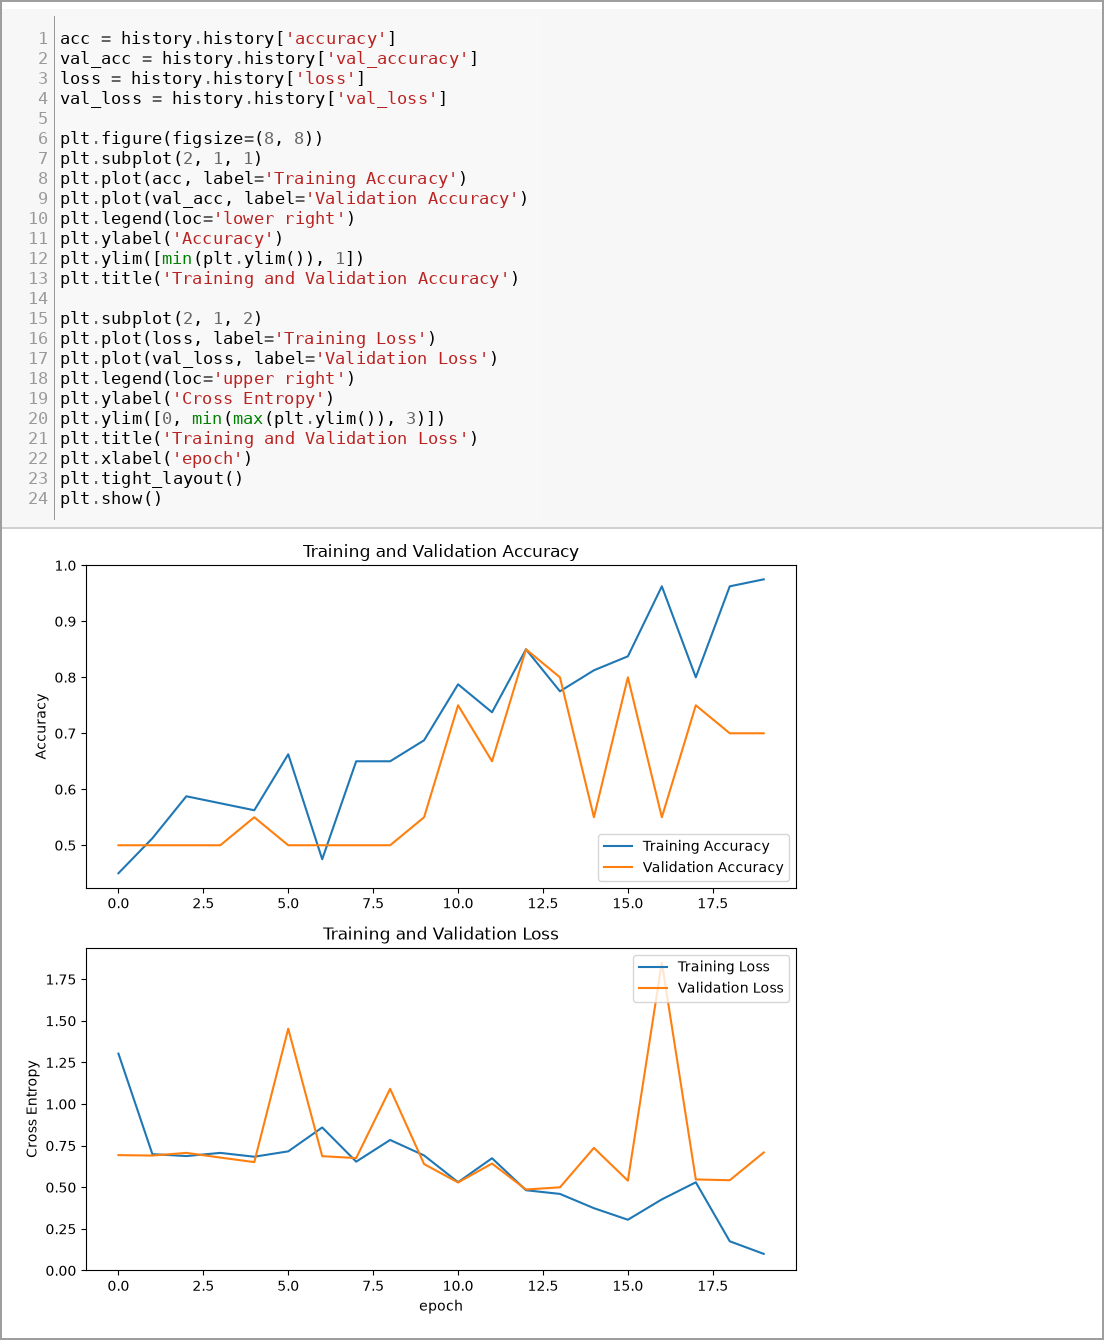
\includegraphics[width=0.72\textwidth]{images/ss-08-grafik-akurasi-loss.png}
	\caption{Grafik akurasi dan loss data latih serta validasi model Dog vs Cat.}
	\label{fig:ss-grafik-dogcat}
\end{figure}

Grafik pada Gambar~\ref{fig:ss-grafik-dogcat} memperlihatkan dua hal. Pertama, kurva validasi sangat bergerigi. Data validasi hanya 20 citra, sehingga satu citra yang salah tebak langsung menggeser akurasi sebesar 0,05; lonjakan \textit{val\_loss} ke 1,85 pada \textit{epoch} 17 juga muncul karena alasan ini. Kedua, setelah \textit{epoch} 13 kurva latih terus naik sedangkan kurva validasi tidak ikut membaik. Selisih akurasi 0,975 berbanding 0,70 di akhir pelatihan adalah tanda \textit{overfitting}. Dengan 25,7 juta parameter dan hanya 80 citra latih, model mudah menghafal data latih. Menurut saya perbaikan yang paling masuk akal adalah menambah jumlah citra, memakai augmentasi data (\textit{flip}, rotasi, \textit{zoom}), atau mengganti \texttt{Flatten} dengan \texttt{GlobalAveragePooling2D} agar parameter lapisan \textit{dense} turun drastis.

\clearpage

\section{Tugas dan Analisis: Klasifikasi Multi-Kelas CIFAR-10}
Untuk tugas, saya memilih dataset CIFAR-10 \cite{krizhevsky2009, cifar-web}. Dataset ini berisi citra berwarna $32 \times 32$ piksel dari 10 kelas: \textit{airplane}, \textit{automobile}, \textit{bird}, \textit{cat}, \textit{deer}, \textit{dog}, \textit{frog}, \textit{horse}, \textit{ship}, dan \textit{truck}. Saya memilih CIFAR-10 karena jumlah datanya cukup besar untuk melihat efek regularisasi dengan jelas, dan beberapa kelasnya mirip satu sama lain (kucing dan anjing, mobil dan truk) sehingga analisis \textit{confusion matrix} jadi lebih menarik.

\subsection{Memuat Dataset}
\begin{figure}[H]
	\centering
	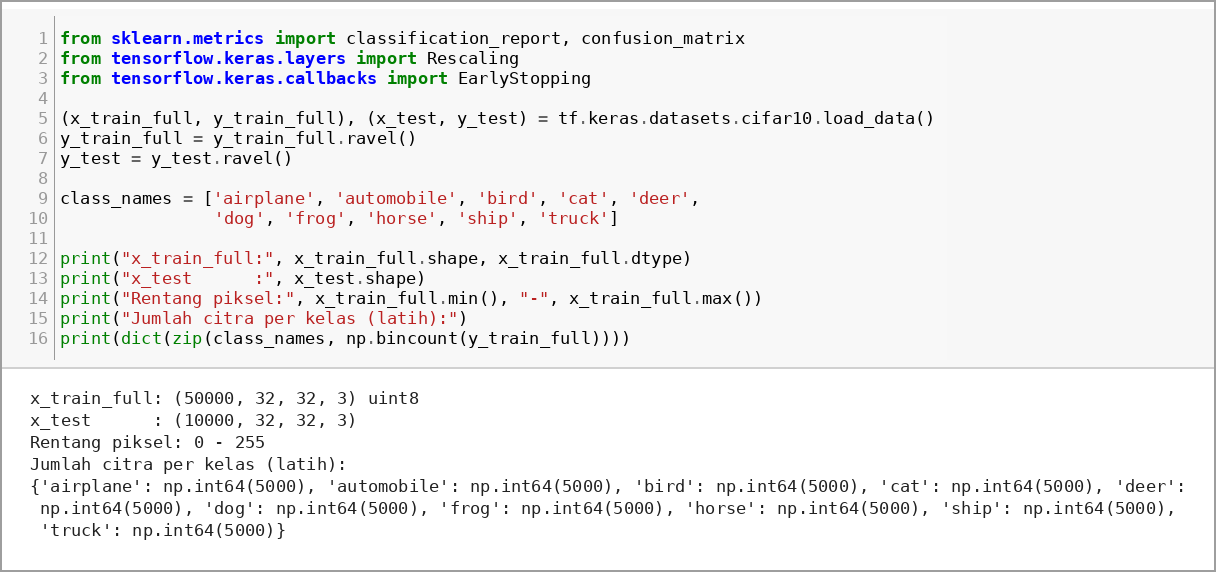
\includegraphics[width=0.85\textwidth]{images/ss-09-cifar-muat.png}
	\caption{Pemuatan dataset CIFAR-10 serta jumlah citra per kelas.}
	\label{fig:ss-cifar-muat}
\end{figure}

Data latih berisi 50.000 citra dan data uji 10.000 citra, bertipe \texttt{uint8} dengan rentang piksel 0 sampai 255. Setiap kelas pada data latih berisi tepat 5.000 citra, jadi dataset ini seimbang dan akurasi bisa dipakai sebagai metrik utama tanpa khawatir bias kelas mayoritas.

\begin{figure}[H]
	\centering
	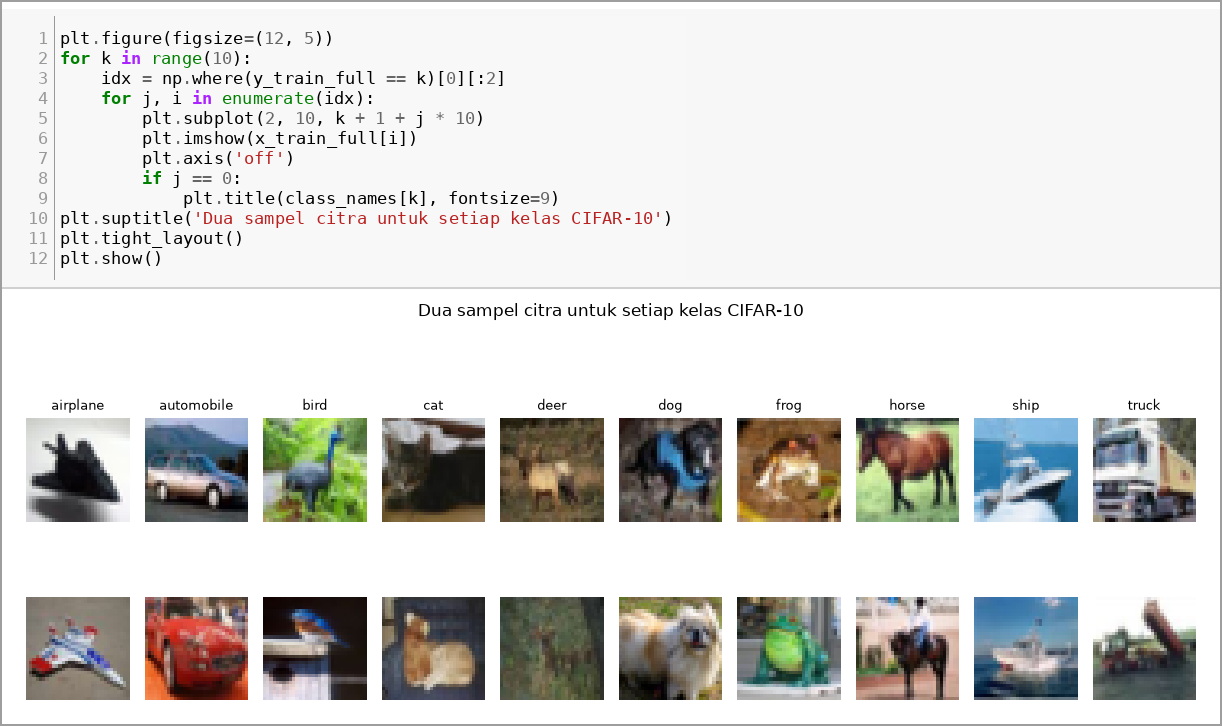
\includegraphics[width=0.9\textwidth]{images/ss-10-cifar-sampel.png}
	\caption{Dua sampel citra untuk setiap kelas CIFAR-10.}
	\label{fig:ss-cifar-sampel}
\end{figure}

Resolusi $32 \times 32$ membuat detail objek sangat kasar. Beberapa citra bahkan sulit saya kenali sendiri tanpa melihat labelnya, terutama kelas hewan berlatar alam.

\subsection{Pembagian Data}
Dari 50.000 citra latih, saya sisihkan 5.000 citra secara acak sebagai data validasi untuk memantau pelatihan dan untuk \textit{early stopping}. Data uji 10.000 citra hanya dipakai satu kali di tahap evaluasi akhir.

\begin{figure}[H]
	\centering
	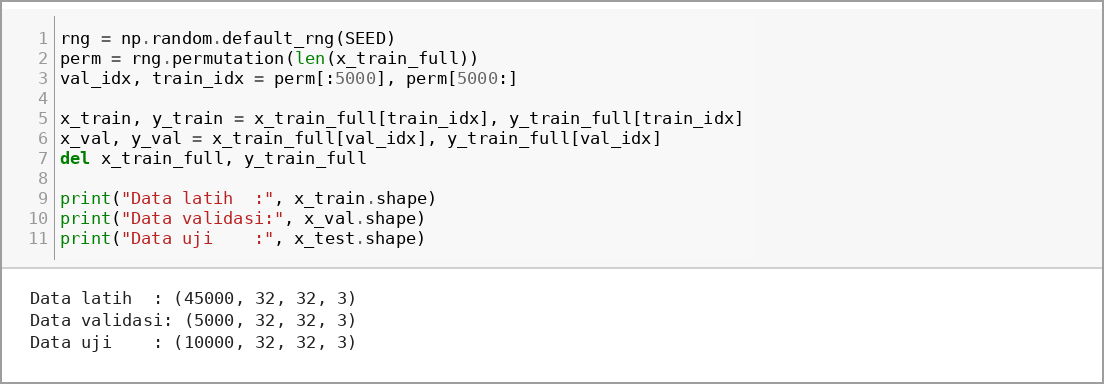
\includegraphics[width=0.8\textwidth]{images/ss-11-cifar-split.png}
	\caption{Pembagian data latih (45.000), validasi (5.000), dan uji (10.000).}
	\label{fig:ss-cifar-split}
\end{figure}

\subsection{Model Pembanding Tanpa Dropout}
Agar pengaruh \textit{dropout} terlihat jelas, saya membuat fungsi \texttt{bangun\_cnn} yang menghasilkan arsitektur yang sama dengan dan tanpa \textit{dropout}. Arsitekturnya terdiri atas lapisan \texttt{Rescaling(1/255)}, tiga blok konvolusi (32, 64, dan 128 filter) yang masing-masing berisi dua \texttt{Conv2D} dan satu \texttt{MaxPooling2D}, lalu \texttt{Flatten}, \texttt{Dense(256)}, dan \texttt{Dense(10)} dengan \textit{softmax}. Rancangan ini mengikuti pola tutorial CNN TensorFlow \cite{tf-cnn}. Model dikompilasi dengan Adam dan \texttt{sparse\_categorical\_crossentropy} karena label CIFAR-10 berupa bilangan bulat 0 sampai 9.

\noindent\begin{minipage}{\linewidth}
\begin{lstlisting}[style=pythonstyle,caption={Fungsi pembangun CNN untuk CIFAR-10.}]
def bangun_cnn(dropout=True):
    m = Sequential(name='cnn_dropout' if dropout else 'cnn_tanpa_dropout')
    m.add(Input(shape=(32, 32, 3)))
    m.add(Rescaling(1. / 255))
    for f, d in [(32, 0.2), (64, 0.3), (128, 0.4)]:
        m.add(Conv2D(f, 3, padding='same', activation='relu'))
        m.add(Conv2D(f, 3, padding='same', activation='relu'))
        m.add(MaxPooling2D((2, 2)))
        if dropout:
            m.add(Dropout(d))
    m.add(Flatten())
    m.add(Dense(256, activation='relu'))
    if dropout:
        m.add(Dropout(0.5))
    m.add(Dense(10, activation='softmax'))
    m.compile(optimizer='adam',
              loss='sparse_categorical_crossentropy',
              metrics=['accuracy'])
    return m
\end{lstlisting}
\end{minipage}

\begin{figure}[H]
	\centering
	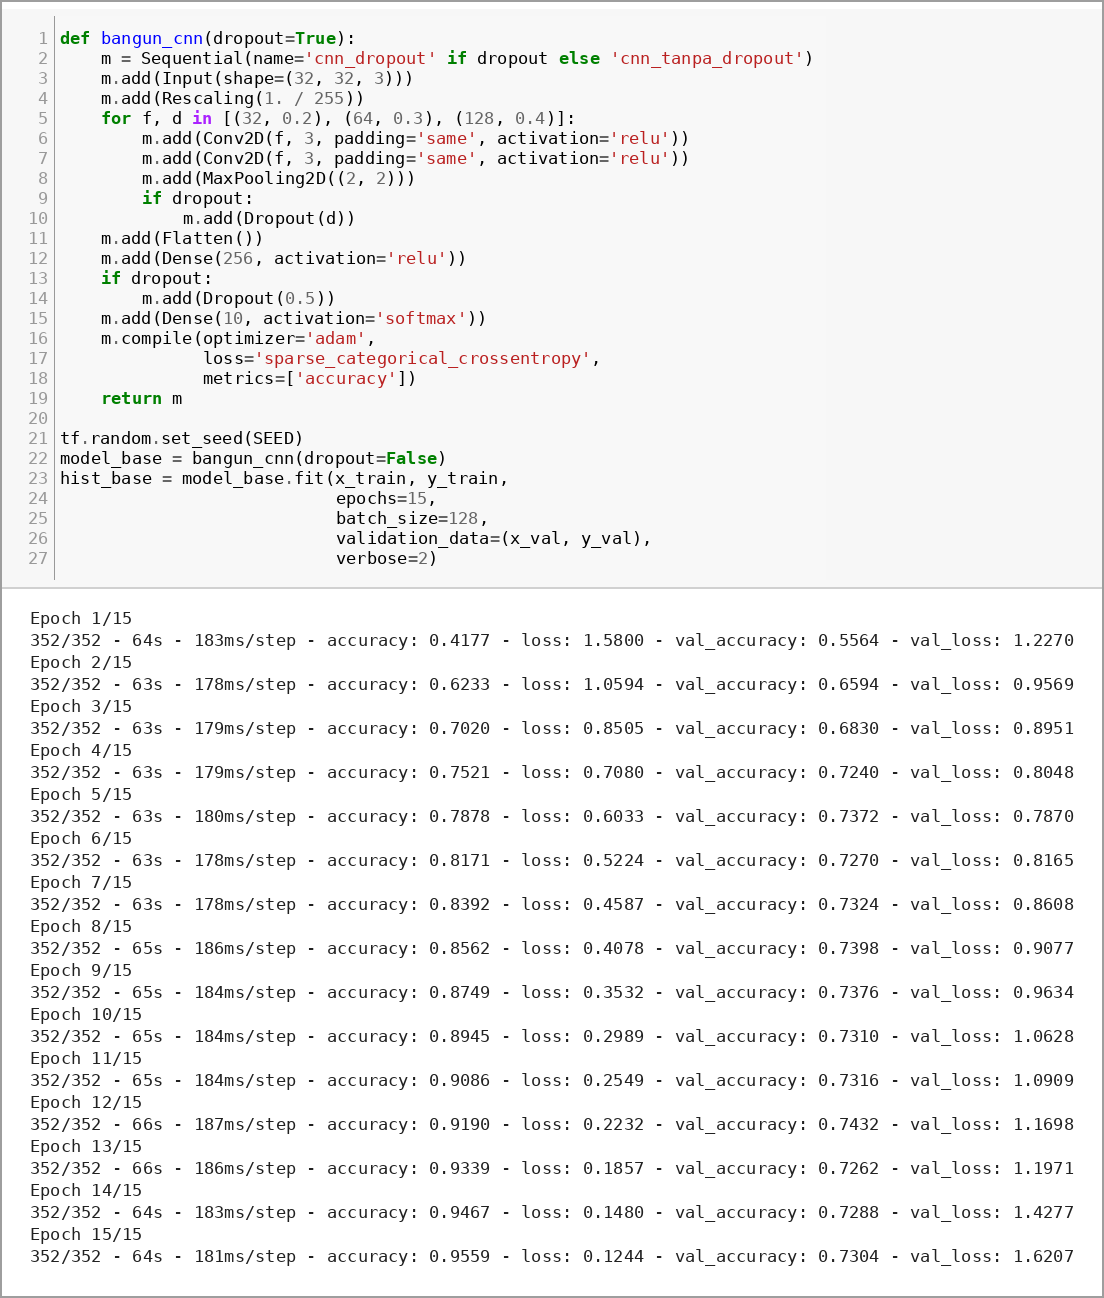
\includegraphics[width=0.78\textwidth]{images/ss-12-cifar-tanpa-dropout.png}
	\caption{Pelatihan model pembanding tanpa \textit{dropout} selama 15 \textit{epoch}.}
	\label{fig:ss-cifar-base}
\end{figure}

Model tanpa \textit{dropout} belajar sangat cepat di data latih: akurasi latih naik dari 0,4177 pada \textit{epoch} 1 menjadi 0,9559 pada \textit{epoch} 15. Namun \textit{val\_loss} terendah sudah tercapai pada \textit{epoch} 5 (0,7870). Setelah itu \textit{val\_loss} justru naik terus sampai 1,6207, sementara akurasi validasi mandek di sekitar 0,73. Pola loss latih turun tetapi loss validasi naik ini adalah gejala \textit{overfitting} yang klasik.

\subsection{Model CNN dengan Regularisasi Dropout}
Model kedua memakai arsitektur yang sama, ditambah \texttt{Dropout} bertingkat: 0,2 setelah blok pertama, 0,3 setelah blok kedua, 0,4 setelah blok ketiga, dan 0,5 setelah \texttt{Dense(256)}. Nilai \textit{dropout} saya buat makin besar di lapisan yang lebih dalam karena jumlah filternya lebih banyak sehingga lebih mudah menghafal. Saya juga memasang \texttt{EarlyStopping} yang memantau \textit{val\_loss} dengan \texttt{patience=5} dan \texttt{restore\_best\_weights=True}.

\begin{figure}[H]
	\centering
	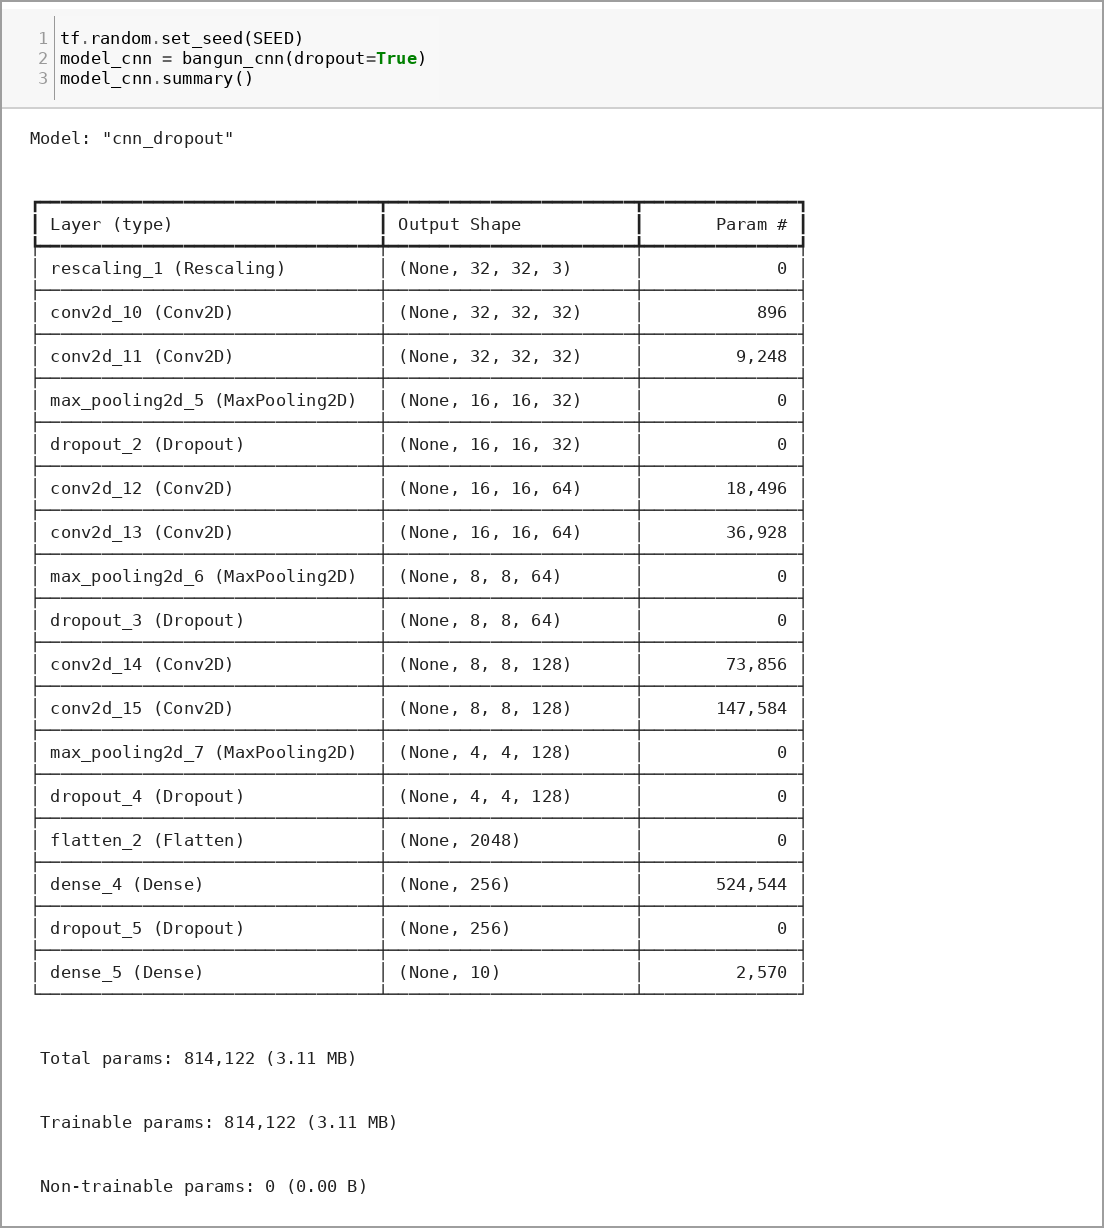
\includegraphics[width=0.75\textwidth]{images/ss-13-cifar-summary-dropout.png}
	\caption{Ringkasan arsitektur CNN dengan \textit{dropout} untuk CIFAR-10.}
	\label{fig:ss-cifar-summary}
\end{figure}

Model ini hanya memiliki 814.122 parameter (3,11 MB), jauh lebih kecil dari model Dog vs Cat. Penyebabnya adalah tiga kali \textit{max pooling} yang memperkecil \textit{feature map} dari $32 \times 32$ menjadi $4 \times 4 \times 128$, sehingga keluaran \texttt{Flatten} hanya 2.048 nilai. Lapisan \textit{dropout} tidak menambah parameter sama sekali.

\begin{figure}[H]
	\centering
	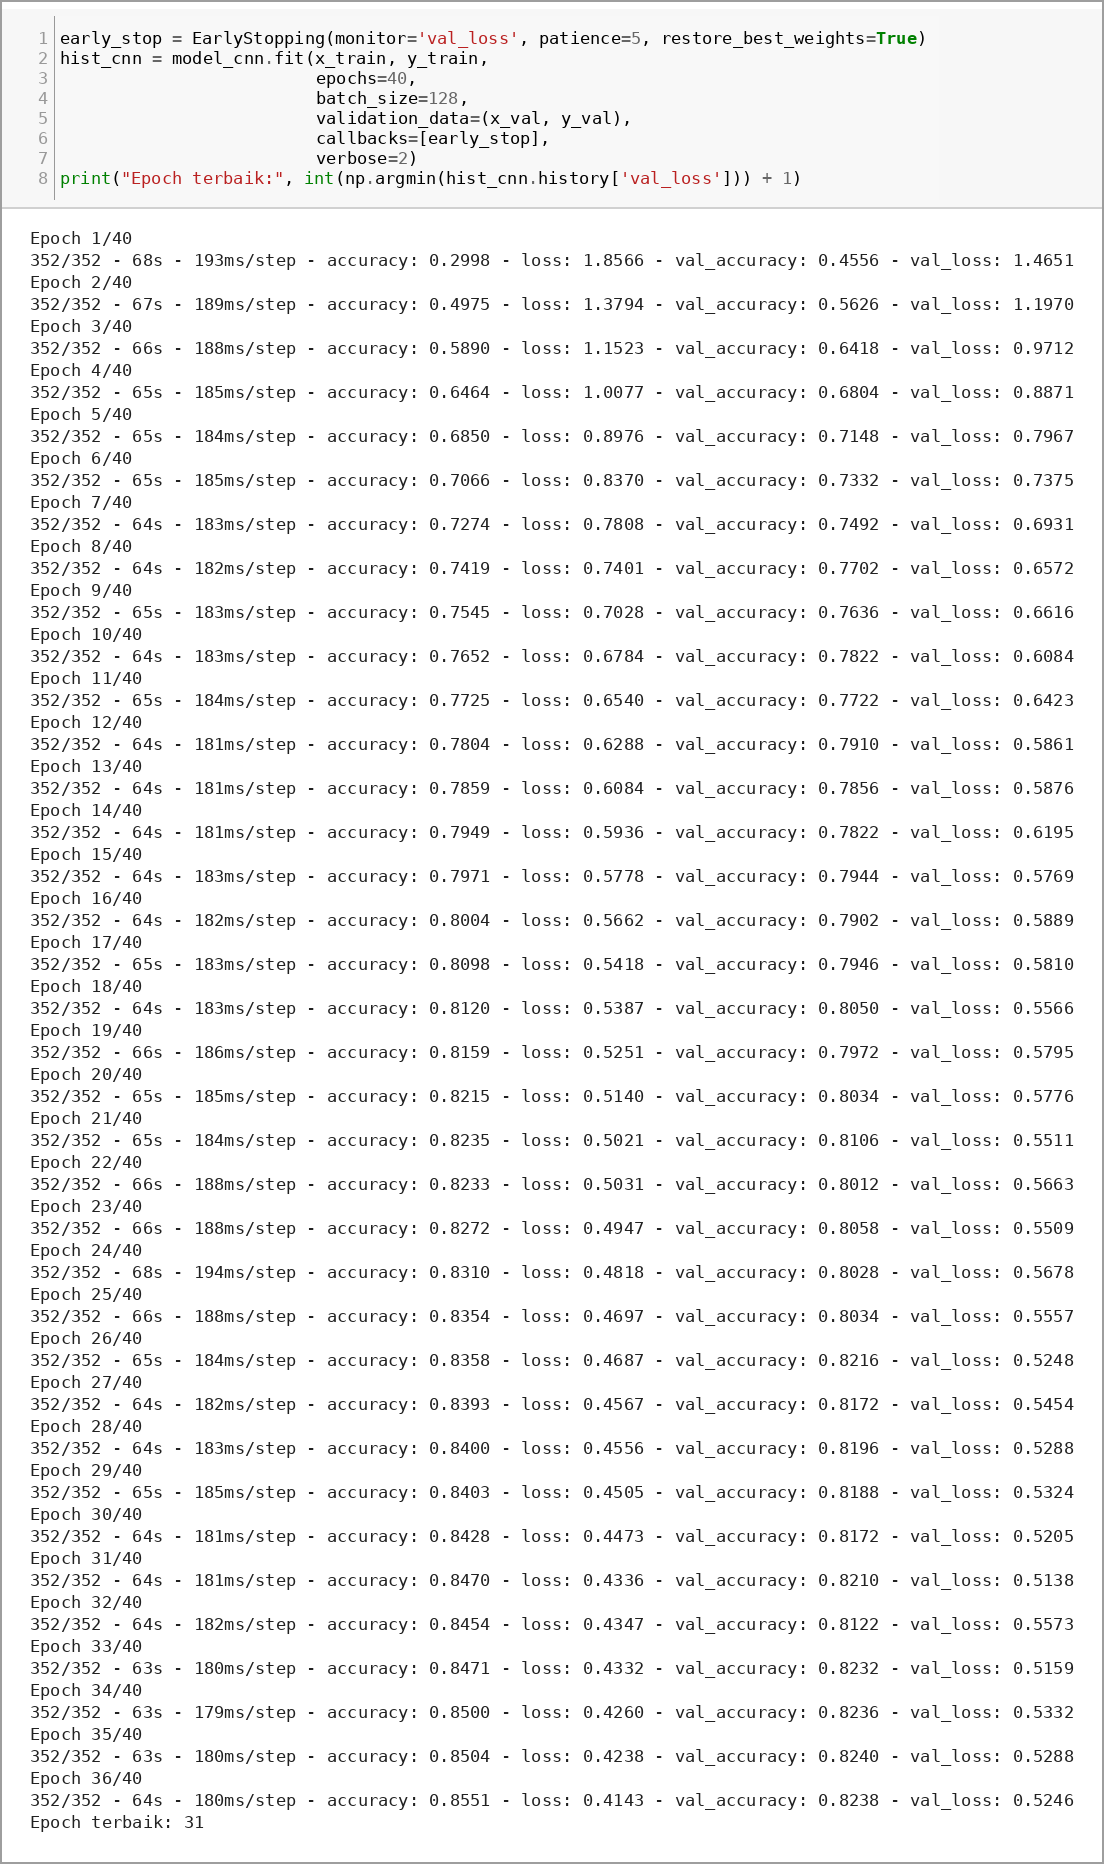
\includegraphics[width=0.72\textwidth]{images/ss-14-cifar-latih-dropout.png}
	\caption{Log pelatihan CNN dengan \textit{dropout} dan \textit{early stopping}.}
	\label{fig:ss-cifar-latih}
\end{figure}

Pelatihan berhenti otomatis pada \textit{epoch} 36 karena \textit{val\_loss} tidak membaik selama lima \textit{epoch} setelah \textit{epoch} 31. Bobot terbaik dari \textit{epoch} 31 (\textit{val\_loss} 0,5138, akurasi validasi 0,8210) dikembalikan ke model. Setiap \textit{epoch} butuh sekitar 64 detik di CPU.

\subsection{Grafik Loss dan Akurasi}
\begin{figure}[H]
	\centering
	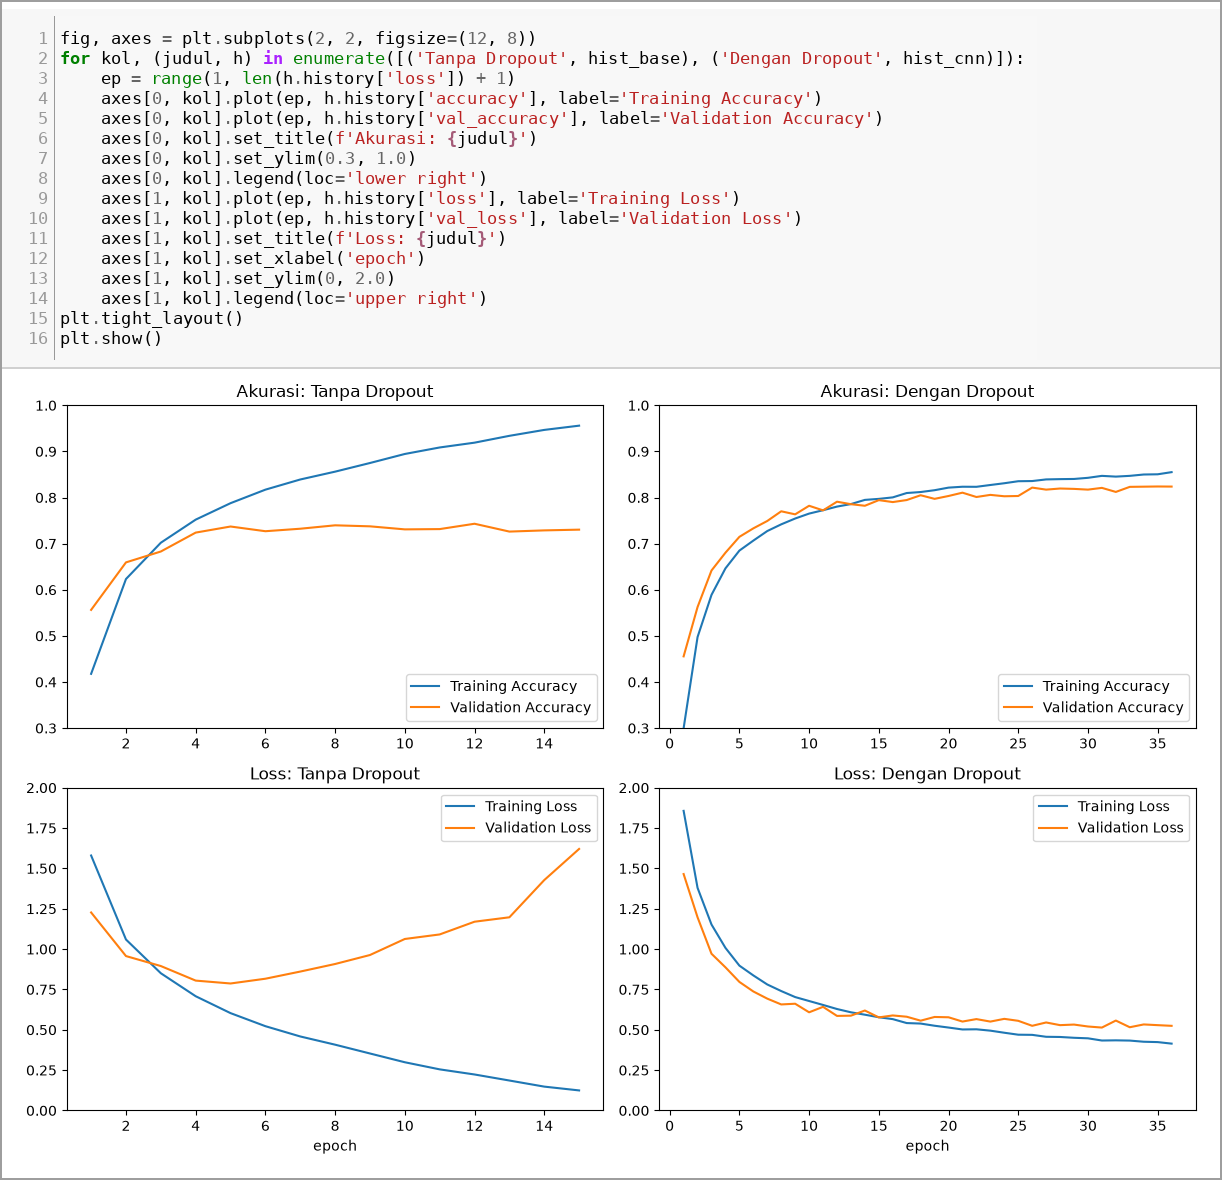
\includegraphics[width=0.92\textwidth]{images/ss-15-cifar-grafik-loss-akurasi.png}
	\caption{Perbandingan kurva akurasi dan loss model tanpa \textit{dropout} (kiri) dan dengan \textit{dropout} (kanan).}
	\label{fig:ss-cifar-grafik}
\end{figure}

Perbedaan kedua model paling jelas terlihat di Gambar~\ref{fig:ss-cifar-grafik}. Pada model tanpa \textit{dropout} (kiri), kurva latih dan validasi berpisah sejak \textit{epoch} 3, dan \textit{val\_loss} membentuk huruf U: turun sampai \textit{epoch} 5 lalu naik terus. Pada model dengan \textit{dropout} (kanan), kedua kurva berjalan berdampingan hampir sepanjang pelatihan. Akurasi validasi bahkan sempat lebih tinggi dari akurasi latih pada 10 \textit{epoch} awal. Hal ini wajar karena akurasi latih dihitung saat \textit{dropout} aktif (sebagian neuron mati), sedangkan validasi dihitung dengan semua neuron aktif. Konsekuensinya, model dengan \textit{dropout} belajar lebih lambat, tetapi akurasi validasinya terus naik sampai sekitar 0,82, jauh di atas batas 0,74 yang dicapai model tanpa \textit{dropout}.

\subsection{Evaluasi pada Data Uji}
\begin{figure}[H]
	\centering
	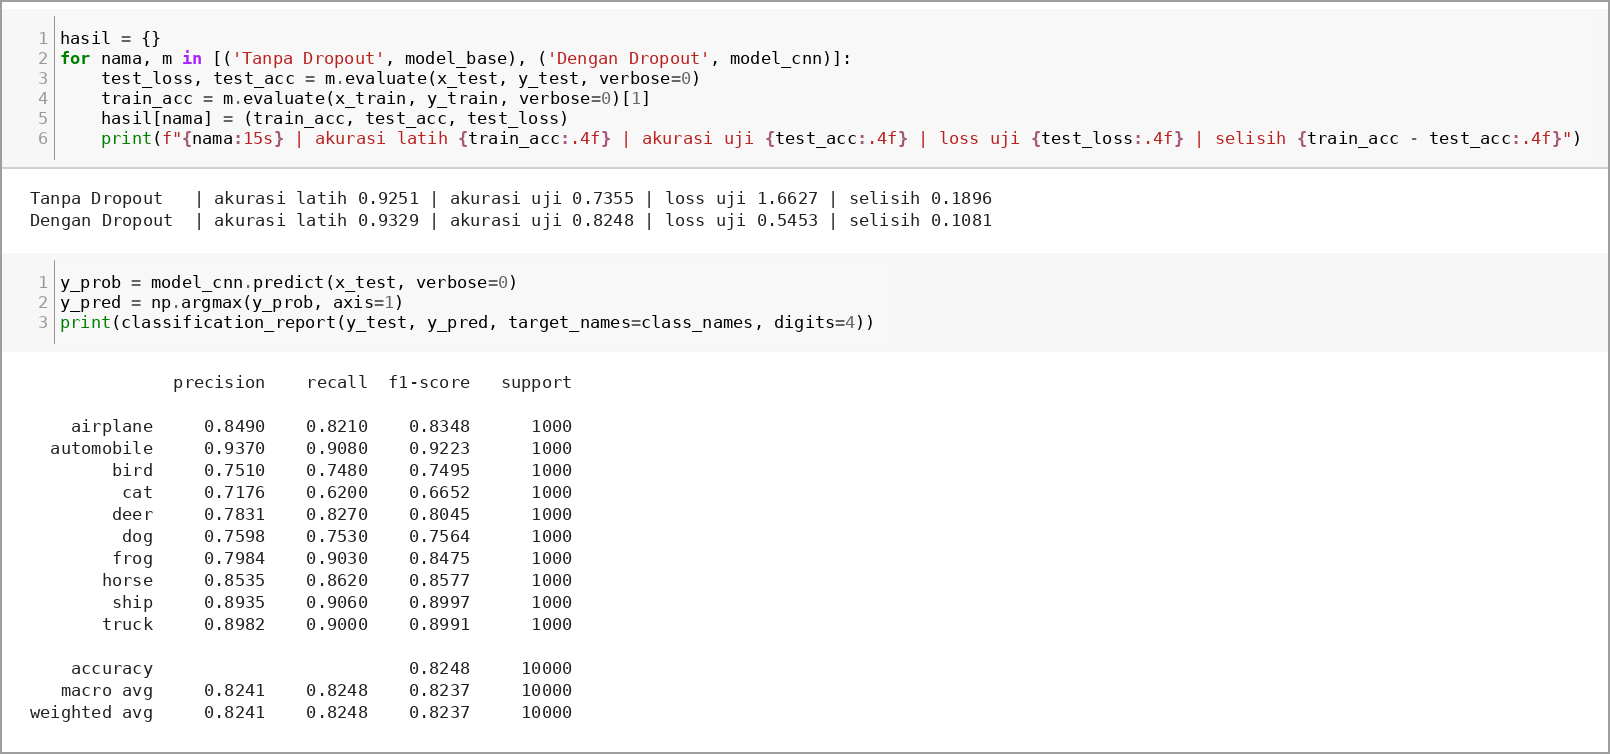
\includegraphics[width=0.92\textwidth]{images/ss-16-cifar-evaluasi-report.png}
	\caption{Perbandingan akurasi kedua model dan \textit{classification report} model dengan \textit{dropout} pada data uji.}
	\label{fig:ss-cifar-report}
\end{figure}

Tabel~\ref{tab:komparasi-cifar} merangkum hasil evaluasi kedua model. Akurasi latih di tabel dihitung ulang dengan \texttt{model.evaluate} (mode inferensi, \textit{dropout} nonaktif), sehingga bisa dibandingkan langsung dengan akurasi uji.

\begin{table}[H]
	\centering
	\caption{Perbandingan performa CNN tanpa dan dengan \textit{dropout} pada CIFAR-10.}
	\label{tab:komparasi-cifar}
	\small
	\begin{tabular}{|l|c|c|c|c|c|}
		\hline
		\textbf{Model}  & \textbf{Epoch} & \textbf{Akurasi Latih} & \textbf{Akurasi Uji} & \textbf{Loss Uji} & \textbf{Selisih} \\
		\hline
		Tanpa \textit{dropout} & 15             & 0,9251                 & 0,7355               & 1,6627            & 0,1896           \\
		\hline
		Dengan \textit{dropout} & 36 (terbaik 31) & 0,9329                 & \textbf{0,8248}      & \textbf{0,5453}   & \textbf{0,1081}  \\
		\hline
	\end{tabular}
\end{table}

\textit{Dropout} menaikkan akurasi uji dari 73,55\% menjadi 82,48\%, atau naik 8,93 poin persentase. Loss uji turun dari 1,6627 menjadi 0,5453. Angka loss uji model tanpa \textit{dropout} yang tinggi menunjukkan model itu terlalu yakin pada prediksi yang salah, efek dari menghafal data latih. Selisih akurasi latih dan uji juga mengecil dari 0,1896 menjadi 0,1081.

Dari \textit{classification report}, kelas dengan F1-\textit{score} tertinggi adalah \textit{automobile} (0,9223), \textit{ship} (0,8997), dan \textit{truck} (0,8991). Ketiganya adalah objek buatan manusia dengan bentuk dan warna yang khas. Kelas terlemah adalah \textit{cat} dengan F1-\textit{score} 0,6652 dan \textit{recall} hanya 0,6200, disusul \textit{bird} (0,7495) dan \textit{dog} (0,7564). Nilai \textit{macro average} dan \textit{weighted average} sama (F1 0,8237) karena jumlah sampel tiap kelas di data uji sama, yaitu 1.000.

\subsection{Confusion Matrix}
\begin{figure}[H]
	\centering
	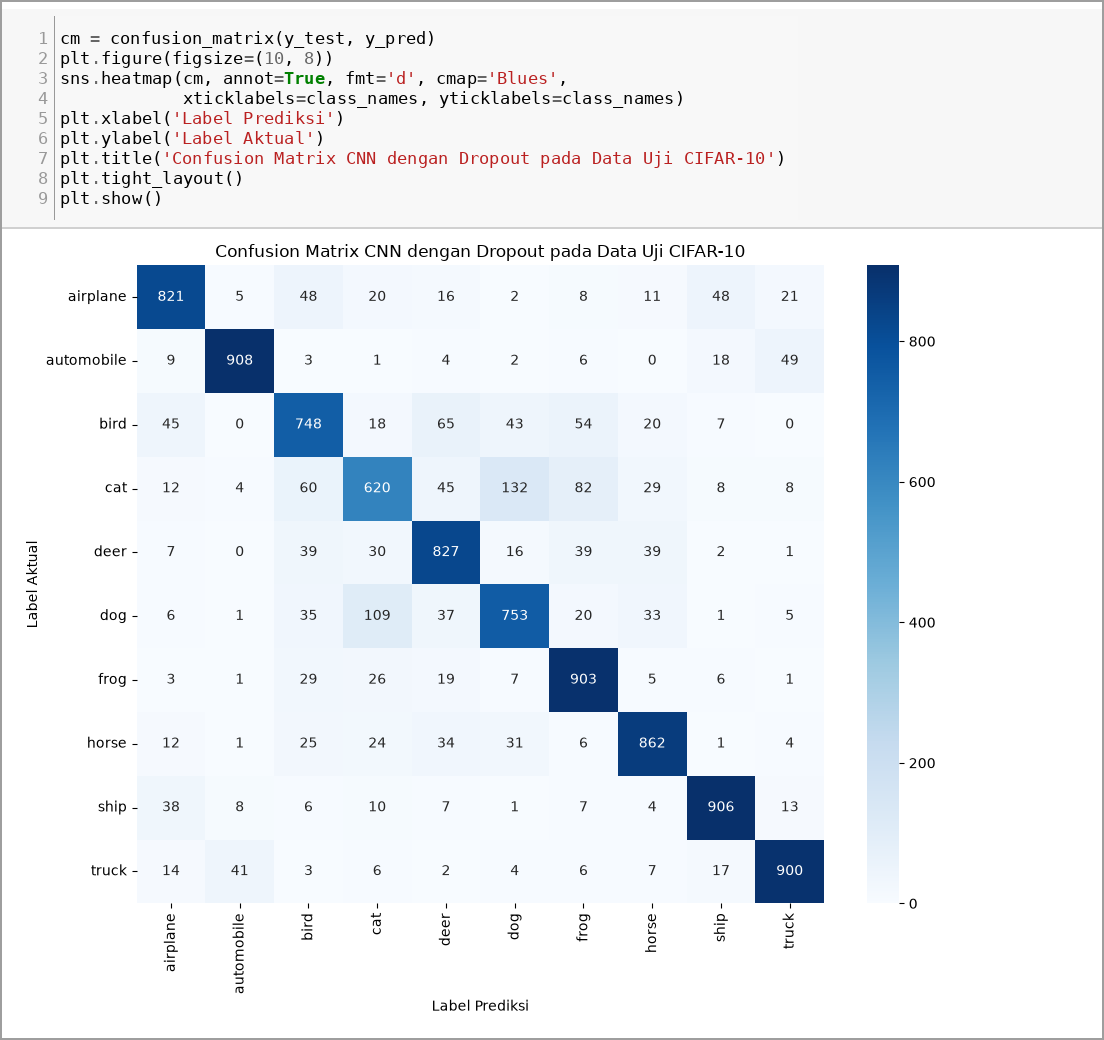
\includegraphics[width=0.85\textwidth]{images/ss-17-cifar-confusion-matrix.png}
	\caption{\textit{Confusion matrix} CNN dengan \textit{dropout} pada 10.000 citra uji CIFAR-10.}
	\label{fig:ss-cifar-cm}
\end{figure}

Diagonal \textit{confusion matrix} pada Gambar~\ref{fig:ss-cifar-cm} menunjukkan jumlah prediksi benar per kelas. Kesalahan di luar diagonal paling banyak mengumpul pada pasangan kelas yang secara visual mirip:
\begin{enumerate}[noitemsep, topsep=2pt, parsep=1pt]
	\item \textbf{\textit{Cat} dan \textit{dog}:} 132 citra kucing diprediksi anjing dan 109 citra anjing diprediksi kucing. Ini pasangan kesalahan terbesar. Pada resolusi $32 \times 32$, bentuk telinga dan moncong yang membedakan keduanya hanya terwakili oleh beberapa piksel.
	\item \textbf{\textit{Automobile} dan \textit{truck}:} 49 mobil diprediksi truk dan 41 truk diprediksi mobil. Keduanya kendaraan beroda dengan latar jalan yang serupa.
	\item \textbf{\textit{Airplane} dengan \textit{bird} dan \textit{ship}:} masing-masing 48 citra pesawat tertukar ke \textit{bird} dan \textit{ship}. Dugaan saya, model ikut memakai warna latar (langit biru atau laut) sebagai petunjuk selain bentuk objeknya.
	\item \textbf{Kelas hewan berlatar alam:} \textit{bird} cukup sering tertukar dengan \textit{deer} (65) dan \textit{frog} (54), dan \textit{cat} tertukar dengan \textit{frog} (82). Latar hijau dan cokelat yang mirip membuat fitur warna kurang bisa membedakan kelas-kelas ini.
\end{enumerate}

\subsection{Contoh Hasil Prediksi}
\begin{figure}[H]
	\centering
	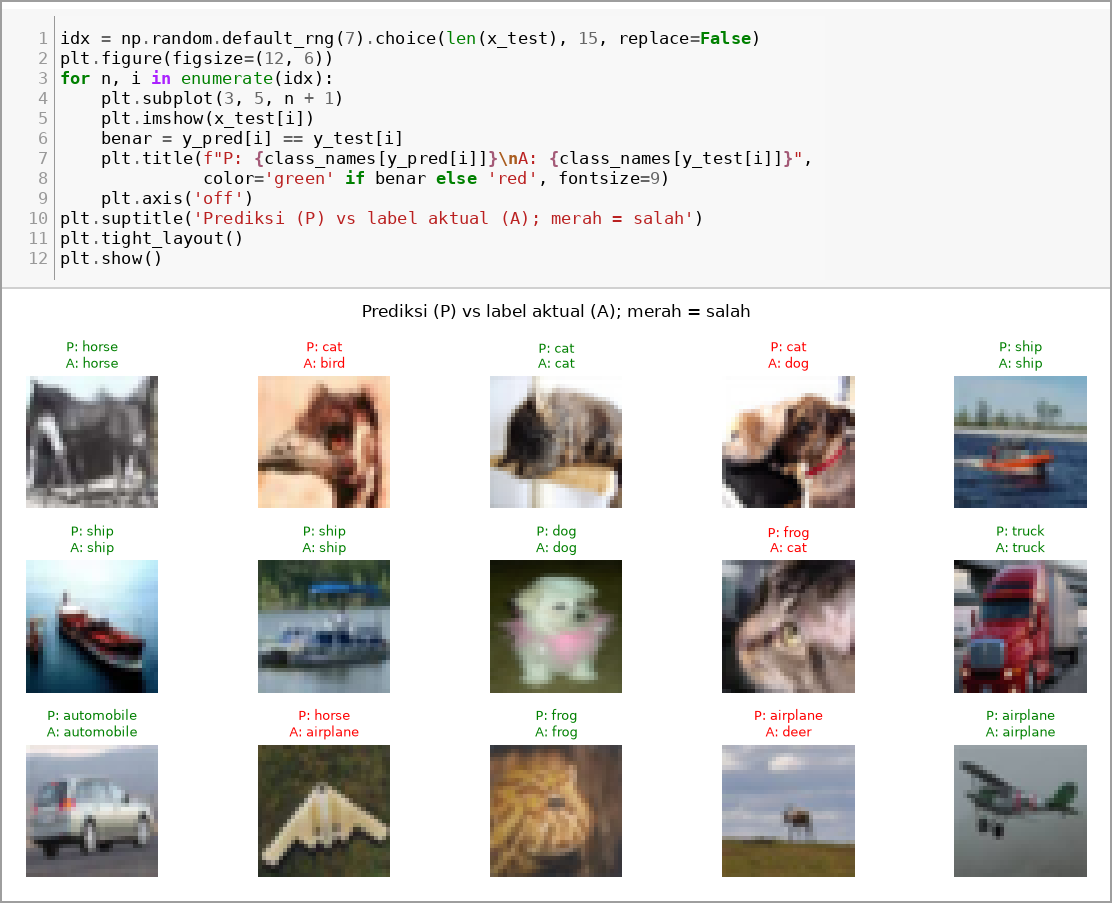
\includegraphics[width=0.85\textwidth]{images/ss-18-cifar-contoh-prediksi.png}
	\caption{Contoh prediksi (P) dan label aktual (A) pada 15 citra uji; judul merah menandakan prediksi salah.}
	\label{fig:ss-cifar-prediksi}
\end{figure}

Dari 15 citra uji yang diambil acak, sebagian besar terklasifikasi benar. Prediksi yang salah umumnya terjadi pada citra yang objeknya kecil, terpotong, atau berlatar ramai, sejalan dengan pola pada \textit{confusion matrix}.

\clearpage

\chapter{Kesimpulan}
Berdasarkan percobaan modul dan tugas yang saya kerjakan pada Pertemuan 9, kesimpulannya adalah sebagai berikut:
\begin{enumerate}[noitemsep, topsep=2pt, parsep=1pt]
	\item Lapisan konvolusi sangat hemat parameter karena memakai \textit{weight sharing}. Pada model Dog vs Cat, empat lapisan \texttt{Conv2D} hanya punya 65.568 parameter, sedangkan satu lapisan \texttt{Dense} setelah \texttt{Flatten} punya 25,69 juta parameter (99,7\% dari total).
	\item Model CNN sederhana pada dataset Dog vs Cat mencapai akurasi validasi tertinggi 0,85 pada \textit{epoch} 13 dan 0,70 di akhir pelatihan, sedangkan akurasi latihnya 0,975. Selisih ini menunjukkan \textit{overfitting} akibat data latih yang hanya 80 citra dibanding parameter yang mencapai 25,7 juta.
	\item Pada CIFAR-10, \textit{dropout} bertingkat (0,2 sampai 0,5) ditambah \textit{early stopping} menaikkan akurasi uji dari 73,55\% menjadi 82,48\% dan menurunkan loss uji dari 1,6627 menjadi 0,5453 dibanding arsitektur yang sama tanpa \textit{dropout}.
	\item Tanpa \textit{dropout}, \textit{val\_loss} sudah mulai naik sejak \textit{epoch} 5. Dengan \textit{dropout}, kurva latih dan validasi berjalan berdampingan sampai \textit{epoch} 31, sehingga model bisa dilatih lebih lama tanpa menghafal data.
	\item \textit{Confusion matrix} memperlihatkan bahwa kesalahan model terkumpul pada kelas yang mirip secara visual, terutama \textit{cat} dan \textit{dog} (241 kesalahan dua arah) serta \textit{automobile} dan \textit{truck} (90 kesalahan dua arah). Kelas \textit{cat} menjadi kelas terlemah dengan F1-\textit{score} 0,6652.
\end{enumerate}

\clearpage

%======================================================================
% DAFTAR PUSTAKA
%======================================================================
\begin{thebibliography}{99}
	\bibitem{colab-notebook} H. R. Prasetya, ``Praktikum 9: Convolutional Neural Network (Notebook),'' Google Colaboratory, 2026. [Online]. Tersedia: \url{https://colab.research.google.com/github/hafidzrizqullahprasetya/PPD/blob/main/pertemuan-9/praktikum-9-convolutional-neural-network.ipynb}.

	\bibitem{goodfellow2016} I. Goodfellow, Y. Bengio, dan A. Courville, \textit{Deep Learning}. Cambridge, MA, USA: MIT Press, 2016. [Online]. Tersedia: \url{https://www.deeplearningbook.org/}.

	\bibitem{han2022} J. Han, J. Pei, dan H. Tong, \textit{Data Mining: Concepts and Techniques}, edisi ke-4. Cambridge, MA, USA: Morgan Kaufmann, 2022.

	\bibitem{keras-conv2d} Keras Team, ``Conv2D layer,'' Keras API Documentation. [Online]. Tersedia: \url{https://keras.io/api/layers/convolution_layers/convolution2d/}.

	\bibitem{keras-dropout} Keras Team, ``Dropout layer,'' Keras API Documentation. [Online]. Tersedia: \url{https://keras.io/api/layers/regularization_layers/dropout/}.

	\bibitem{krizhevsky2009} A. Krizhevsky, ``Learning multiple layers of features from tiny images,'' University of Toronto, Tech. Rep., 2009. [Online]. Tersedia: \url{https://www.cs.toronto.edu/~kriz/learning-features-2009-TR.pdf}.

	\bibitem{cifar-web} A. Krizhevsky, ``The CIFAR-10 dataset,'' University of Toronto. [Online]. Tersedia: \url{https://www.cs.toronto.edu/~kriz/cifar.html}.

	\bibitem{krizhevsky2012} A. Krizhevsky, I. Sutskever, dan G. E. Hinton, ``ImageNet classification with deep convolutional neural networks,'' dalam \textit{Advances in Neural Information Processing Systems 25 (NIPS 2012)}, 2012, hlm. 1097 sampai 1105. [Online]. Tersedia: \url{https://proceedings.neurips.cc/paper/2012/hash/c399862d3b9d6b76c8436e924a68c45b-Abstract.html}.

	\bibitem{lecun1998} Y. LeCun, L. Bottou, Y. Bengio, dan P. Haffner, ``Gradient-based learning applied to document recognition,'' \textit{Proceedings of the IEEE}, vol. 86, no. 11, hlm. 2278 sampai 2324, 1998.

	\bibitem{oshea2015} K. O'Shea dan R. Nash, ``An introduction to convolutional neural networks,'' \textit{arXiv preprint arXiv:1511.08458}, 2015. [Online]. Tersedia: \url{https://arxiv.org/abs/1511.08458}.

	\bibitem{srivastava2014} N. Srivastava, G. Hinton, A. Krizhevsky, I. Sutskever, dan R. Salakhutdinov, ``Dropout: A simple way to prevent neural networks from overfitting,'' \textit{Journal of Machine Learning Research}, vol. 15, no. 56, hlm. 1929 sampai 1958, 2014. [Online]. Tersedia: \url{https://jmlr.org/papers/v15/srivastava14a.html}.

	\bibitem{tf-cnn} TensorFlow, ``Convolutional Neural Network (CNN),'' TensorFlow Tutorials. [Online]. Tersedia: \url{https://www.tensorflow.org/tutorials/images/cnn}.
\end{thebibliography}

\end{document}
